% Options for packages loaded elsewhere
\PassOptionsToPackage{unicode}{hyperref}
\PassOptionsToPackage{hyphens}{url}
\PassOptionsToPackage{dvipsnames,svgnames,x11names}{xcolor}
%
\documentclass[
  letterpaper,
  DIV=11,
  numbers=noendperiod]{scrartcl}

\usepackage{amsmath,amssymb}
\usepackage{lmodern}
\usepackage{iftex}
\ifPDFTeX
  \usepackage[T1]{fontenc}
  \usepackage[utf8]{inputenc}
  \usepackage{textcomp} % provide euro and other symbols
\else % if luatex or xetex
  \usepackage{unicode-math}
  \defaultfontfeatures{Scale=MatchLowercase}
  \defaultfontfeatures[\rmfamily]{Ligatures=TeX,Scale=1}
\fi
% Use upquote if available, for straight quotes in verbatim environments
\IfFileExists{upquote.sty}{\usepackage{upquote}}{}
\IfFileExists{microtype.sty}{% use microtype if available
  \usepackage[]{microtype}
  \UseMicrotypeSet[protrusion]{basicmath} % disable protrusion for tt fonts
}{}
\makeatletter
\@ifundefined{KOMAClassName}{% if non-KOMA class
  \IfFileExists{parskip.sty}{%
    \usepackage{parskip}
  }{% else
    \setlength{\parindent}{0pt}
    \setlength{\parskip}{6pt plus 2pt minus 1pt}}
}{% if KOMA class
  \KOMAoptions{parskip=half}}
\makeatother
\usepackage{xcolor}
\usepackage[normalem]{ulem}
\setlength{\emergencystretch}{3em} % prevent overfull lines
\setcounter{secnumdepth}{-\maxdimen} % remove section numbering
% Make \paragraph and \subparagraph free-standing
\ifx\paragraph\undefined\else
  \let\oldparagraph\paragraph
  \renewcommand{\paragraph}[1]{\oldparagraph{#1}\mbox{}}
\fi
\ifx\subparagraph\undefined\else
  \let\oldsubparagraph\subparagraph
  \renewcommand{\subparagraph}[1]{\oldsubparagraph{#1}\mbox{}}
\fi

\usepackage{color}
\usepackage{fancyvrb}
\newcommand{\VerbBar}{|}
\newcommand{\VERB}{\Verb[commandchars=\\\{\}]}
\DefineVerbatimEnvironment{Highlighting}{Verbatim}{commandchars=\\\{\}}
% Add ',fontsize=\small' for more characters per line
\usepackage{framed}
\definecolor{shadecolor}{RGB}{241,243,245}
\newenvironment{Shaded}{\begin{snugshade}}{\end{snugshade}}
\newcommand{\AlertTok}[1]{\textcolor[rgb]{0.68,0.00,0.00}{#1}}
\newcommand{\AnnotationTok}[1]{\textcolor[rgb]{0.37,0.37,0.37}{#1}}
\newcommand{\AttributeTok}[1]{\textcolor[rgb]{0.40,0.45,0.13}{#1}}
\newcommand{\BaseNTok}[1]{\textcolor[rgb]{0.68,0.00,0.00}{#1}}
\newcommand{\BuiltInTok}[1]{\textcolor[rgb]{0.00,0.23,0.31}{#1}}
\newcommand{\CharTok}[1]{\textcolor[rgb]{0.13,0.47,0.30}{#1}}
\newcommand{\CommentTok}[1]{\textcolor[rgb]{0.37,0.37,0.37}{#1}}
\newcommand{\CommentVarTok}[1]{\textcolor[rgb]{0.37,0.37,0.37}{\textit{#1}}}
\newcommand{\ConstantTok}[1]{\textcolor[rgb]{0.56,0.35,0.01}{#1}}
\newcommand{\ControlFlowTok}[1]{\textcolor[rgb]{0.00,0.23,0.31}{#1}}
\newcommand{\DataTypeTok}[1]{\textcolor[rgb]{0.68,0.00,0.00}{#1}}
\newcommand{\DecValTok}[1]{\textcolor[rgb]{0.68,0.00,0.00}{#1}}
\newcommand{\DocumentationTok}[1]{\textcolor[rgb]{0.37,0.37,0.37}{\textit{#1}}}
\newcommand{\ErrorTok}[1]{\textcolor[rgb]{0.68,0.00,0.00}{#1}}
\newcommand{\ExtensionTok}[1]{\textcolor[rgb]{0.00,0.23,0.31}{#1}}
\newcommand{\FloatTok}[1]{\textcolor[rgb]{0.68,0.00,0.00}{#1}}
\newcommand{\FunctionTok}[1]{\textcolor[rgb]{0.28,0.35,0.67}{#1}}
\newcommand{\ImportTok}[1]{\textcolor[rgb]{0.00,0.46,0.62}{#1}}
\newcommand{\InformationTok}[1]{\textcolor[rgb]{0.37,0.37,0.37}{#1}}
\newcommand{\KeywordTok}[1]{\textcolor[rgb]{0.00,0.23,0.31}{#1}}
\newcommand{\NormalTok}[1]{\textcolor[rgb]{0.00,0.23,0.31}{#1}}
\newcommand{\OperatorTok}[1]{\textcolor[rgb]{0.37,0.37,0.37}{#1}}
\newcommand{\OtherTok}[1]{\textcolor[rgb]{0.00,0.23,0.31}{#1}}
\newcommand{\PreprocessorTok}[1]{\textcolor[rgb]{0.68,0.00,0.00}{#1}}
\newcommand{\RegionMarkerTok}[1]{\textcolor[rgb]{0.00,0.23,0.31}{#1}}
\newcommand{\SpecialCharTok}[1]{\textcolor[rgb]{0.37,0.37,0.37}{#1}}
\newcommand{\SpecialStringTok}[1]{\textcolor[rgb]{0.13,0.47,0.30}{#1}}
\newcommand{\StringTok}[1]{\textcolor[rgb]{0.13,0.47,0.30}{#1}}
\newcommand{\VariableTok}[1]{\textcolor[rgb]{0.07,0.07,0.07}{#1}}
\newcommand{\VerbatimStringTok}[1]{\textcolor[rgb]{0.13,0.47,0.30}{#1}}
\newcommand{\WarningTok}[1]{\textcolor[rgb]{0.37,0.37,0.37}{\textit{#1}}}

\providecommand{\tightlist}{%
  \setlength{\itemsep}{0pt}\setlength{\parskip}{0pt}}\usepackage{longtable,booktabs,array}
\usepackage{calc} % for calculating minipage widths
% Correct order of tables after \paragraph or \subparagraph
\usepackage{etoolbox}
\makeatletter
\patchcmd\longtable{\par}{\if@noskipsec\mbox{}\fi\par}{}{}
\makeatother
% Allow footnotes in longtable head/foot
\IfFileExists{footnotehyper.sty}{\usepackage{footnotehyper}}{\usepackage{footnote}}
\makesavenoteenv{longtable}
\usepackage{graphicx}
\makeatletter
\def\maxwidth{\ifdim\Gin@nat@width>\linewidth\linewidth\else\Gin@nat@width\fi}
\def\maxheight{\ifdim\Gin@nat@height>\textheight\textheight\else\Gin@nat@height\fi}
\makeatother
% Scale images if necessary, so that they will not overflow the page
% margins by default, and it is still possible to overwrite the defaults
% using explicit options in \includegraphics[width, height, ...]{}
\setkeys{Gin}{width=\maxwidth,height=\maxheight,keepaspectratio}
% Set default figure placement to htbp
\makeatletter
\def\fps@figure{htbp}
\makeatother

\KOMAoption{captions}{tableheading}
\makeatletter
\makeatother
\makeatletter
\makeatother
\makeatletter
\@ifpackageloaded{caption}{}{\usepackage{caption}}
\AtBeginDocument{%
\ifdefined\contentsname
  \renewcommand*\contentsname{Table of contents}
\else
  \newcommand\contentsname{Table of contents}
\fi
\ifdefined\listfigurename
  \renewcommand*\listfigurename{List of Figures}
\else
  \newcommand\listfigurename{List of Figures}
\fi
\ifdefined\listtablename
  \renewcommand*\listtablename{List of Tables}
\else
  \newcommand\listtablename{List of Tables}
\fi
\ifdefined\figurename
  \renewcommand*\figurename{Figure}
\else
  \newcommand\figurename{Figure}
\fi
\ifdefined\tablename
  \renewcommand*\tablename{Table}
\else
  \newcommand\tablename{Table}
\fi
}
\@ifpackageloaded{float}{}{\usepackage{float}}
\floatstyle{ruled}
\@ifundefined{c@chapter}{\newfloat{codelisting}{h}{lop}}{\newfloat{codelisting}{h}{lop}[chapter]}
\floatname{codelisting}{Listing}
\newcommand*\listoflistings{\listof{codelisting}{List of Listings}}
\makeatother
\makeatletter
\@ifpackageloaded{caption}{}{\usepackage{caption}}
\@ifpackageloaded{subcaption}{}{\usepackage{subcaption}}
\makeatother
\makeatletter
\@ifpackageloaded{tcolorbox}{}{\usepackage[many]{tcolorbox}}
\makeatother
\makeatletter
\@ifundefined{shadecolor}{\definecolor{shadecolor}{rgb}{.97, .97, .97}}
\makeatother
\makeatletter
\makeatother
\ifLuaTeX
  \usepackage{selnolig}  % disable illegal ligatures
\fi
\IfFileExists{bookmark.sty}{\usepackage{bookmark}}{\usepackage{hyperref}}
\IfFileExists{xurl.sty}{\usepackage{xurl}}{} % add URL line breaks if available
\urlstyle{same} % disable monospaced font for URLs
\hypersetup{
  pdftitle={Quarto Presentations},
  colorlinks=true,
  linkcolor={blue},
  filecolor={Maroon},
  citecolor={Blue},
  urlcolor={Blue},
  pdfcreator={LaTeX via pandoc}}

\title{Quarto Presentations}
\usepackage{etoolbox}
\makeatletter
\providecommand{\subtitle}[1]{% add subtitle to \maketitle
  \apptocmd{\@title}{\par {\large #1 \par}}{}{}
}
\makeatother
\subtitle{Create beautiful interactive slide decks with Reveal.js}
\author{}
\date{}

\begin{document}
\maketitle
\ifdefined\Shaded\renewenvironment{Shaded}{\begin{tcolorbox}[frame hidden, borderline west={3pt}{0pt}{shadecolor}, boxrule=0pt, breakable, interior hidden, sharp corners, enhanced]}{\end{tcolorbox}}\fi

\hypertarget{overview}{%
\subsection{Overview}\label{overview}}

What I will present today:

\begin{itemize}
\tightlist
\item
  How to write, share, and present code and text using R and Quarto
\item
  How to render code and text into different output formats (including
  presentations and APA style articles in word)
\item
  How to use Zotero with R
\item
  How to collaborate using Git and GitHub (only introduction)
\end{itemize}

\ldots and some other stuff

\hypertarget{resources}{%
\subsection{Resources}\label{resources}}

\begin{itemize}
\tightlist
\item
  many of the Quarto-specific slides adapted from
  \href{https://github.com/jthomasmock/quarto-2hr-webinar}{Thomas Mock's
  presentation}
\end{itemize}

\hypertarget{workshop-prep-do-it-now}{%
\subsection{Workshop Prep (do it now!)}\label{workshop-prep-do-it-now}}

\begin{itemize}
\tightlist
\item
  Are you on the latest version of RStudio
  i.e.~\href{https://www.rstudio.com/products/rstudio/download/\#download}{\texttt{v2022.07.1}
  or later}?
\end{itemize}

\begin{Shaded}
\begin{Highlighting}[]
\NormalTok{pkg\_list }\OtherTok{\textless{}{-}} \FunctionTok{c}\NormalTok{(}
  \StringTok{"tidyverse"}\NormalTok{, }\StringTok{"gt"}\NormalTok{, }\StringTok{"gtExtras"}\NormalTok{, }\StringTok{"reactable"}\NormalTok{, }\StringTok{"ggiraph"}\NormalTok{, }\StringTok{"here"}\NormalTok{, }\StringTok{"quarto"}\NormalTok{,}
  \StringTok{"rmarkdown"}\NormalTok{, }\StringTok{"gtsummary"}\NormalTok{, }\StringTok{"palmerpenguins"}\NormalTok{, }\StringTok{"fs"}\NormalTok{, }\StringTok{"skimr"}
\NormalTok{  )}
\FunctionTok{install.packages}\NormalTok{(pkg\_list)}
\end{Highlighting}
\end{Shaded}

\hypertarget{hello-quarto}{%
\subsection{Hello Quarto}\label{hello-quarto}}

\begin{quote}
\hypertarget{quarto-is-an-open-source-scientific-and-technical-publishing-system-built-on-pandoc}{%
\subsubsection{\texorpdfstring{Quarto\textsuperscript{®} is an
open-source scientific and technical publishing system built on
\href{https://pandoc.org/}{Pandoc}}{Quarto® is an open-source scientific and technical publishing system built on Pandoc}}\label{quarto-is-an-open-source-scientific-and-technical-publishing-system-built-on-pandoc}}

. . .
\end{quote}

\begin{quote}
You can weave together narrative text and code to produce elegantly
formatted output as documents, web pages, blog posts, books and more.
\end{quote}

\hypertarget{how-does-rmarkdown-work}{%
\subsection{How does RMarkdown work?}\label{how-does-rmarkdown-work}}

\begin{itemize}
\tightlist
\item
  \texttt{knitr} started in 2011, RMarkdown in 2014
\end{itemize}

\begin{figure}

{\centering 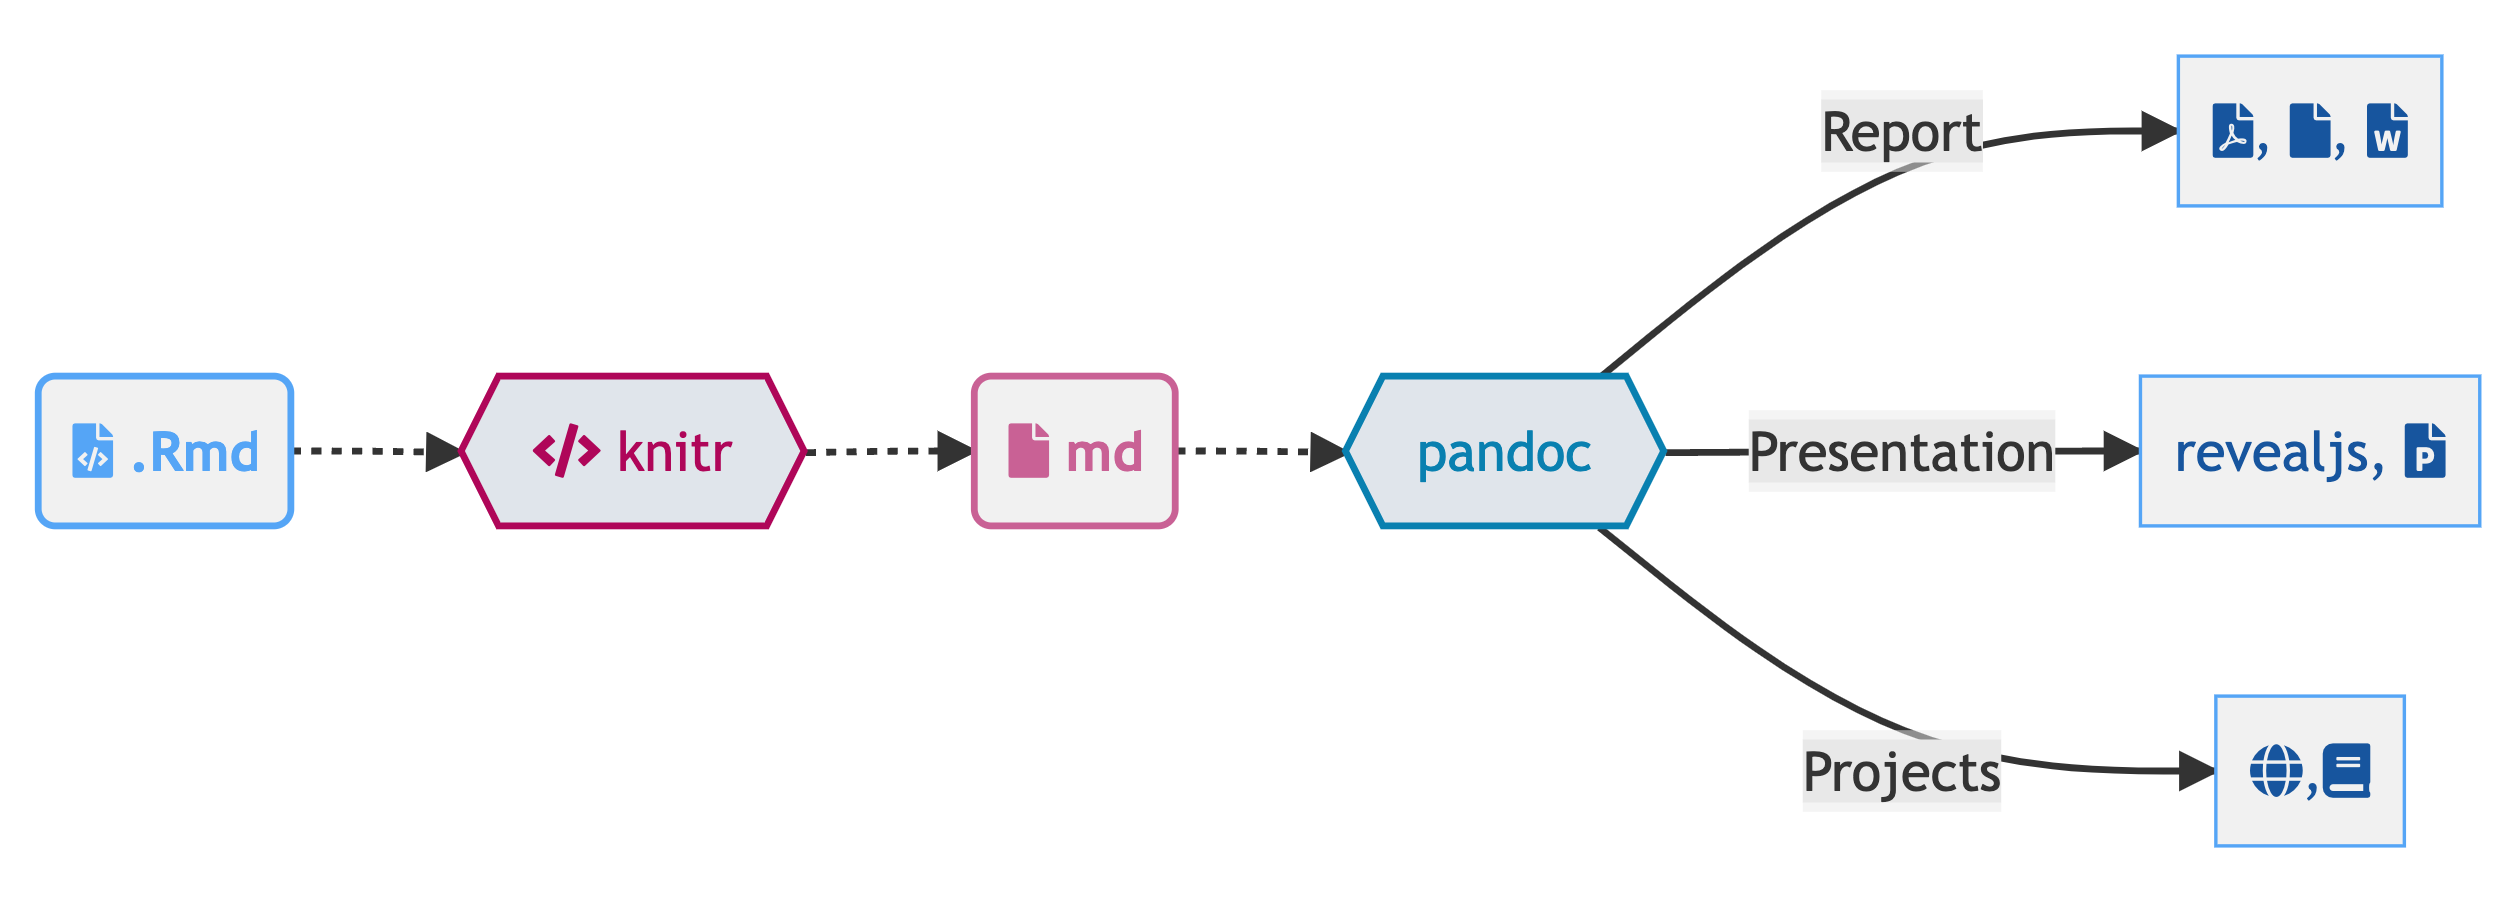
\includegraphics{images/rmd-knitr.png}

}

\end{figure}

\hypertarget{quarto-more-than-just-knitr}{%
\subsection{\texorpdfstring{Quarto, more than \emph{just}
\texttt{knitr}}{Quarto, more than just knitr}}\label{quarto-more-than-just-knitr}}

. . .

We learned from 10 years of literate programming with \texttt{knitr} +
\texttt{rmarkdown}

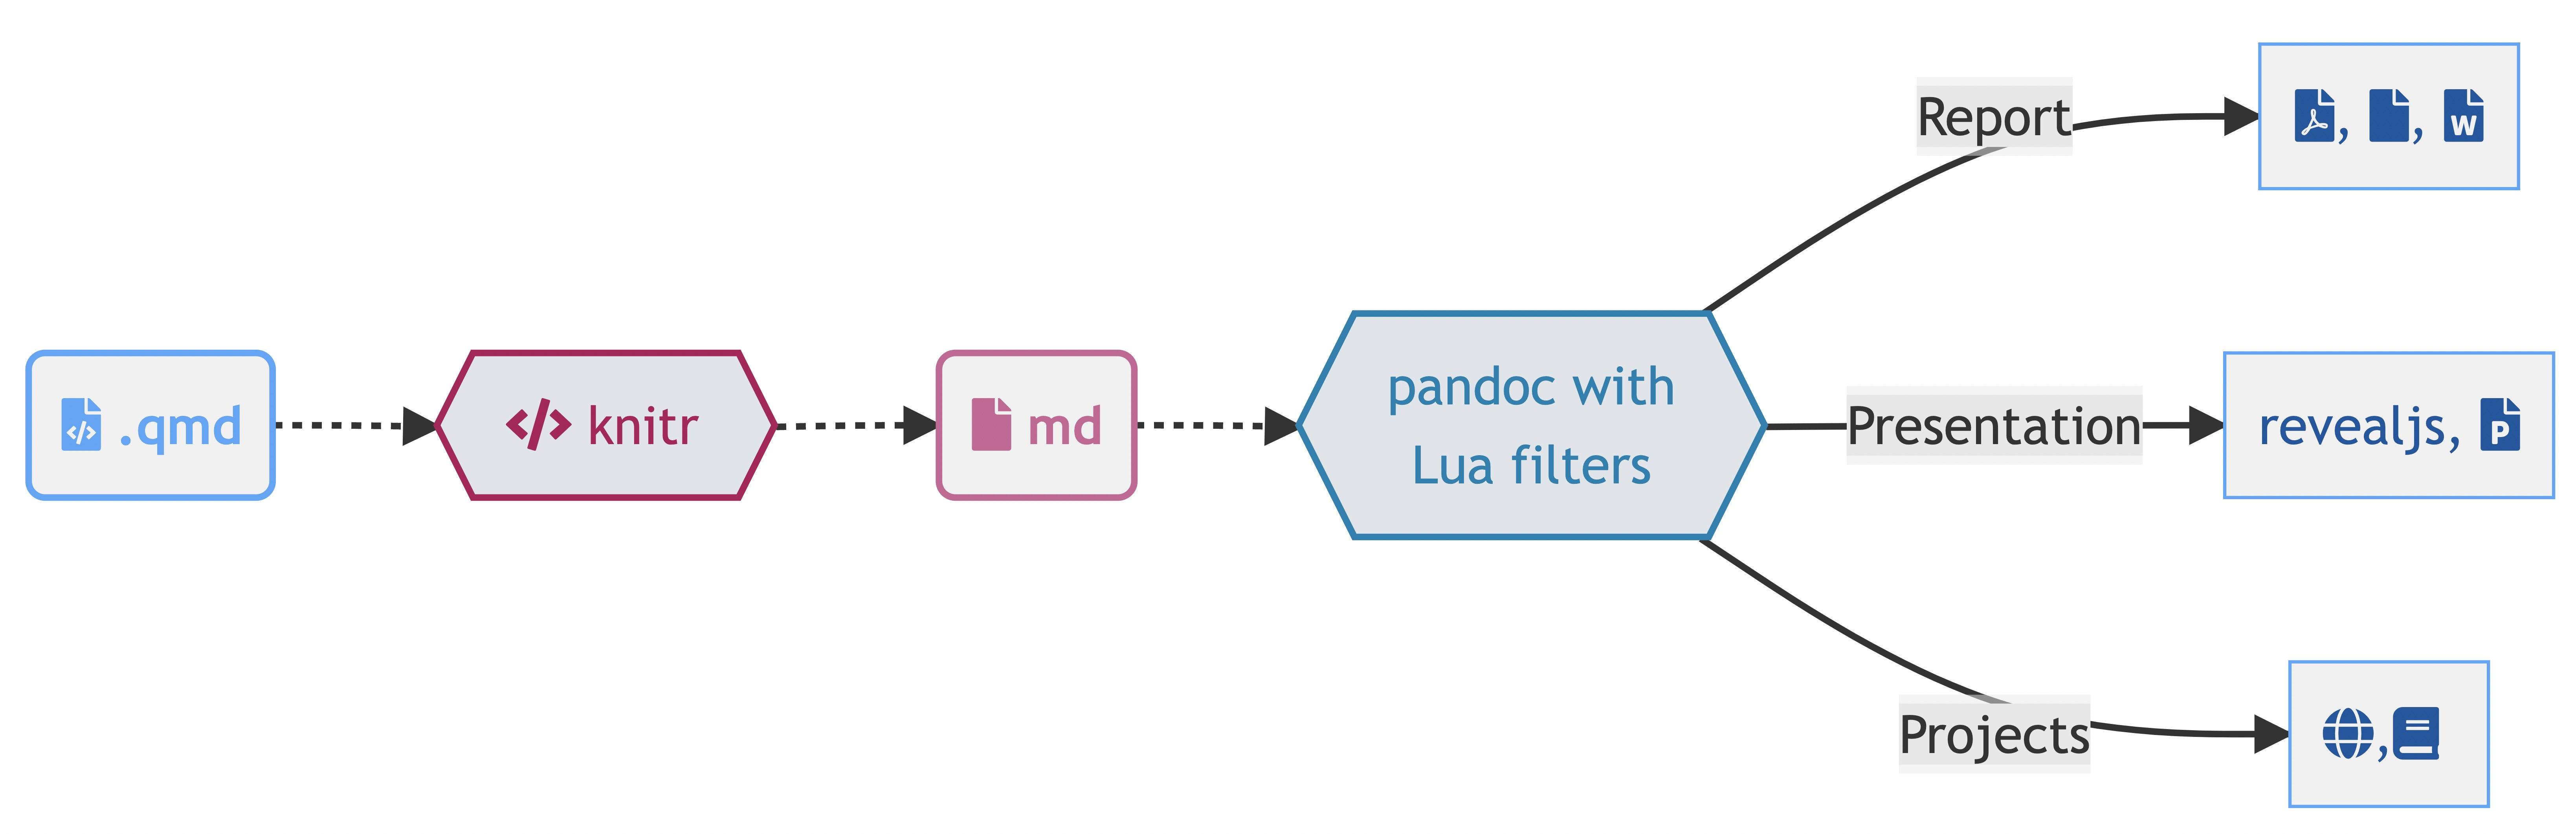
\includegraphics{images/qmd-knitr.jpeg}

\hypertarget{quarto-more-than-just-knitr-1}{%
\subsection{\texorpdfstring{Quarto, more than \emph{just}
\texttt{knitr}}{Quarto, more than just knitr}}\label{quarto-more-than-just-knitr-1}}

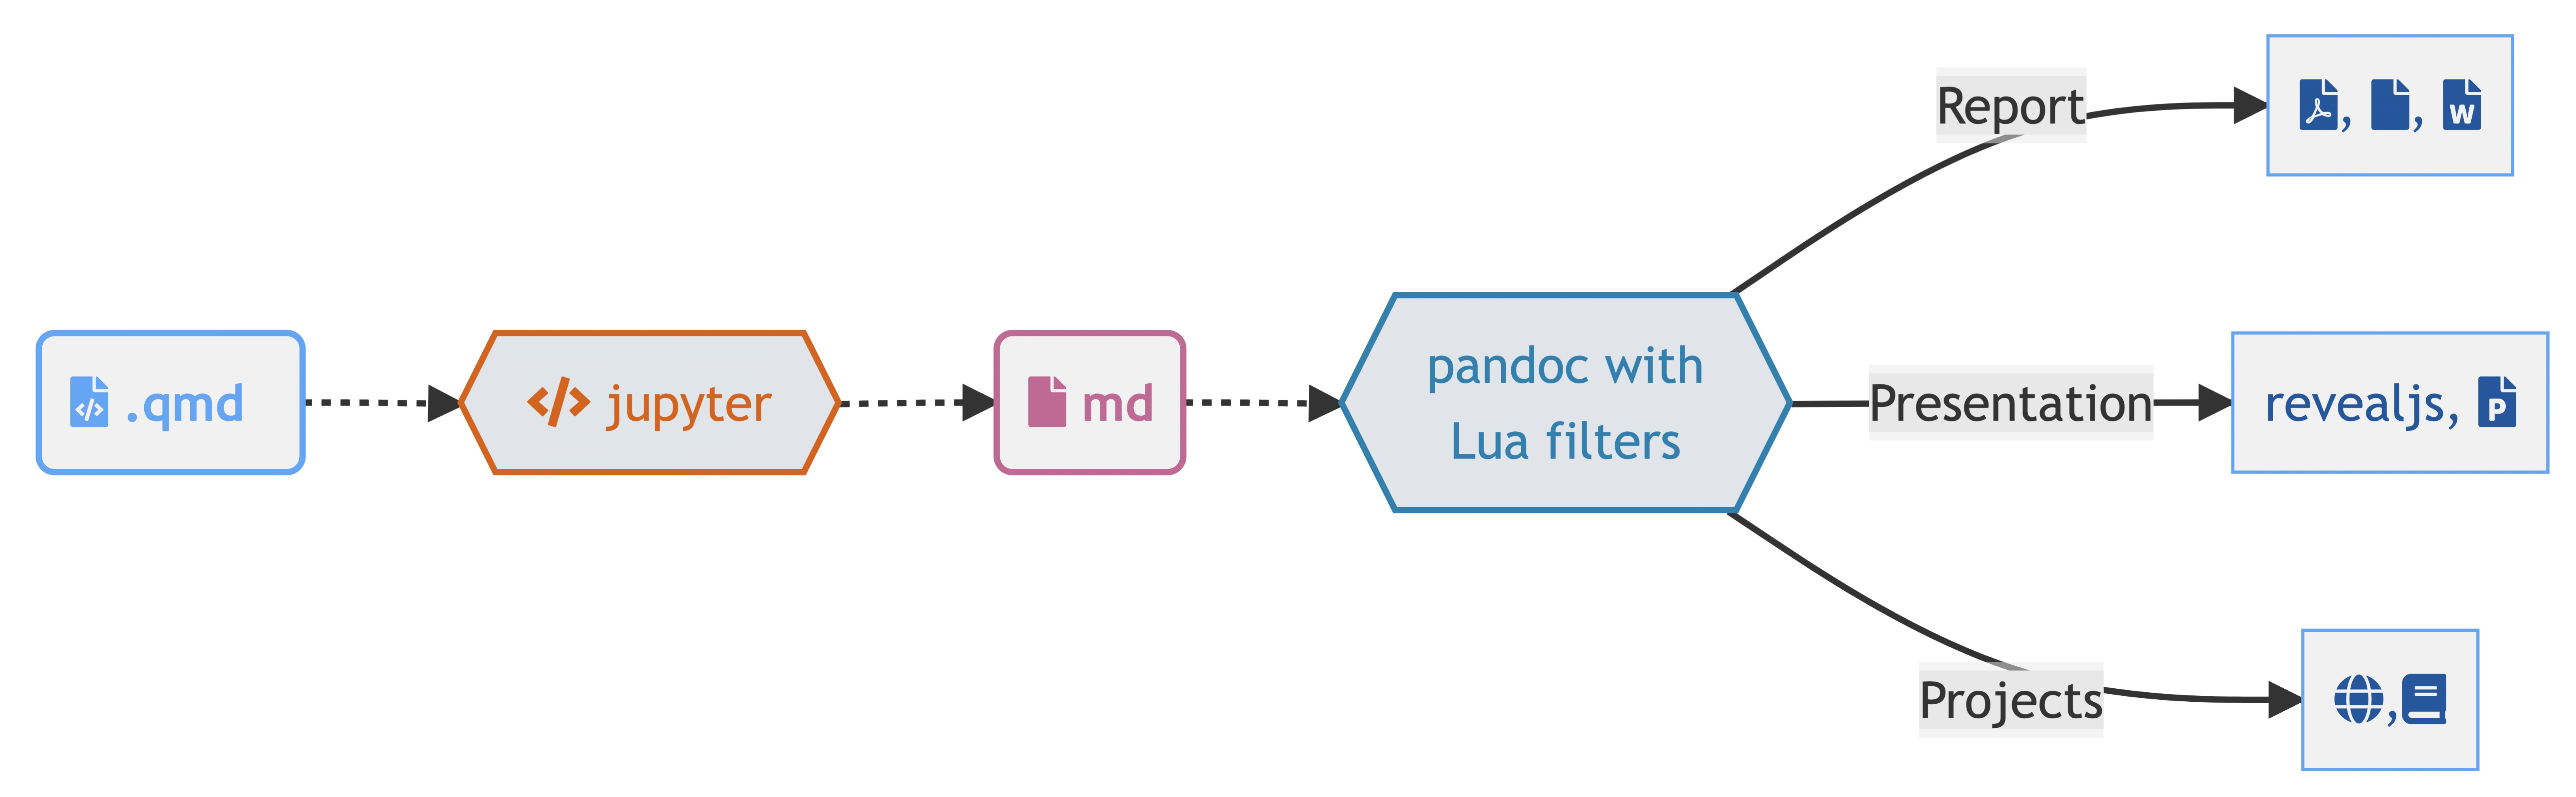
\includegraphics{images/qmd-jupyter.jpeg}

\hypertarget{quarto-more-than-just-knitr-2}{%
\subsection{\texorpdfstring{Quarto, more than \emph{just}
\texttt{knitr}}{Quarto, more than just knitr}}\label{quarto-more-than-just-knitr-2}}

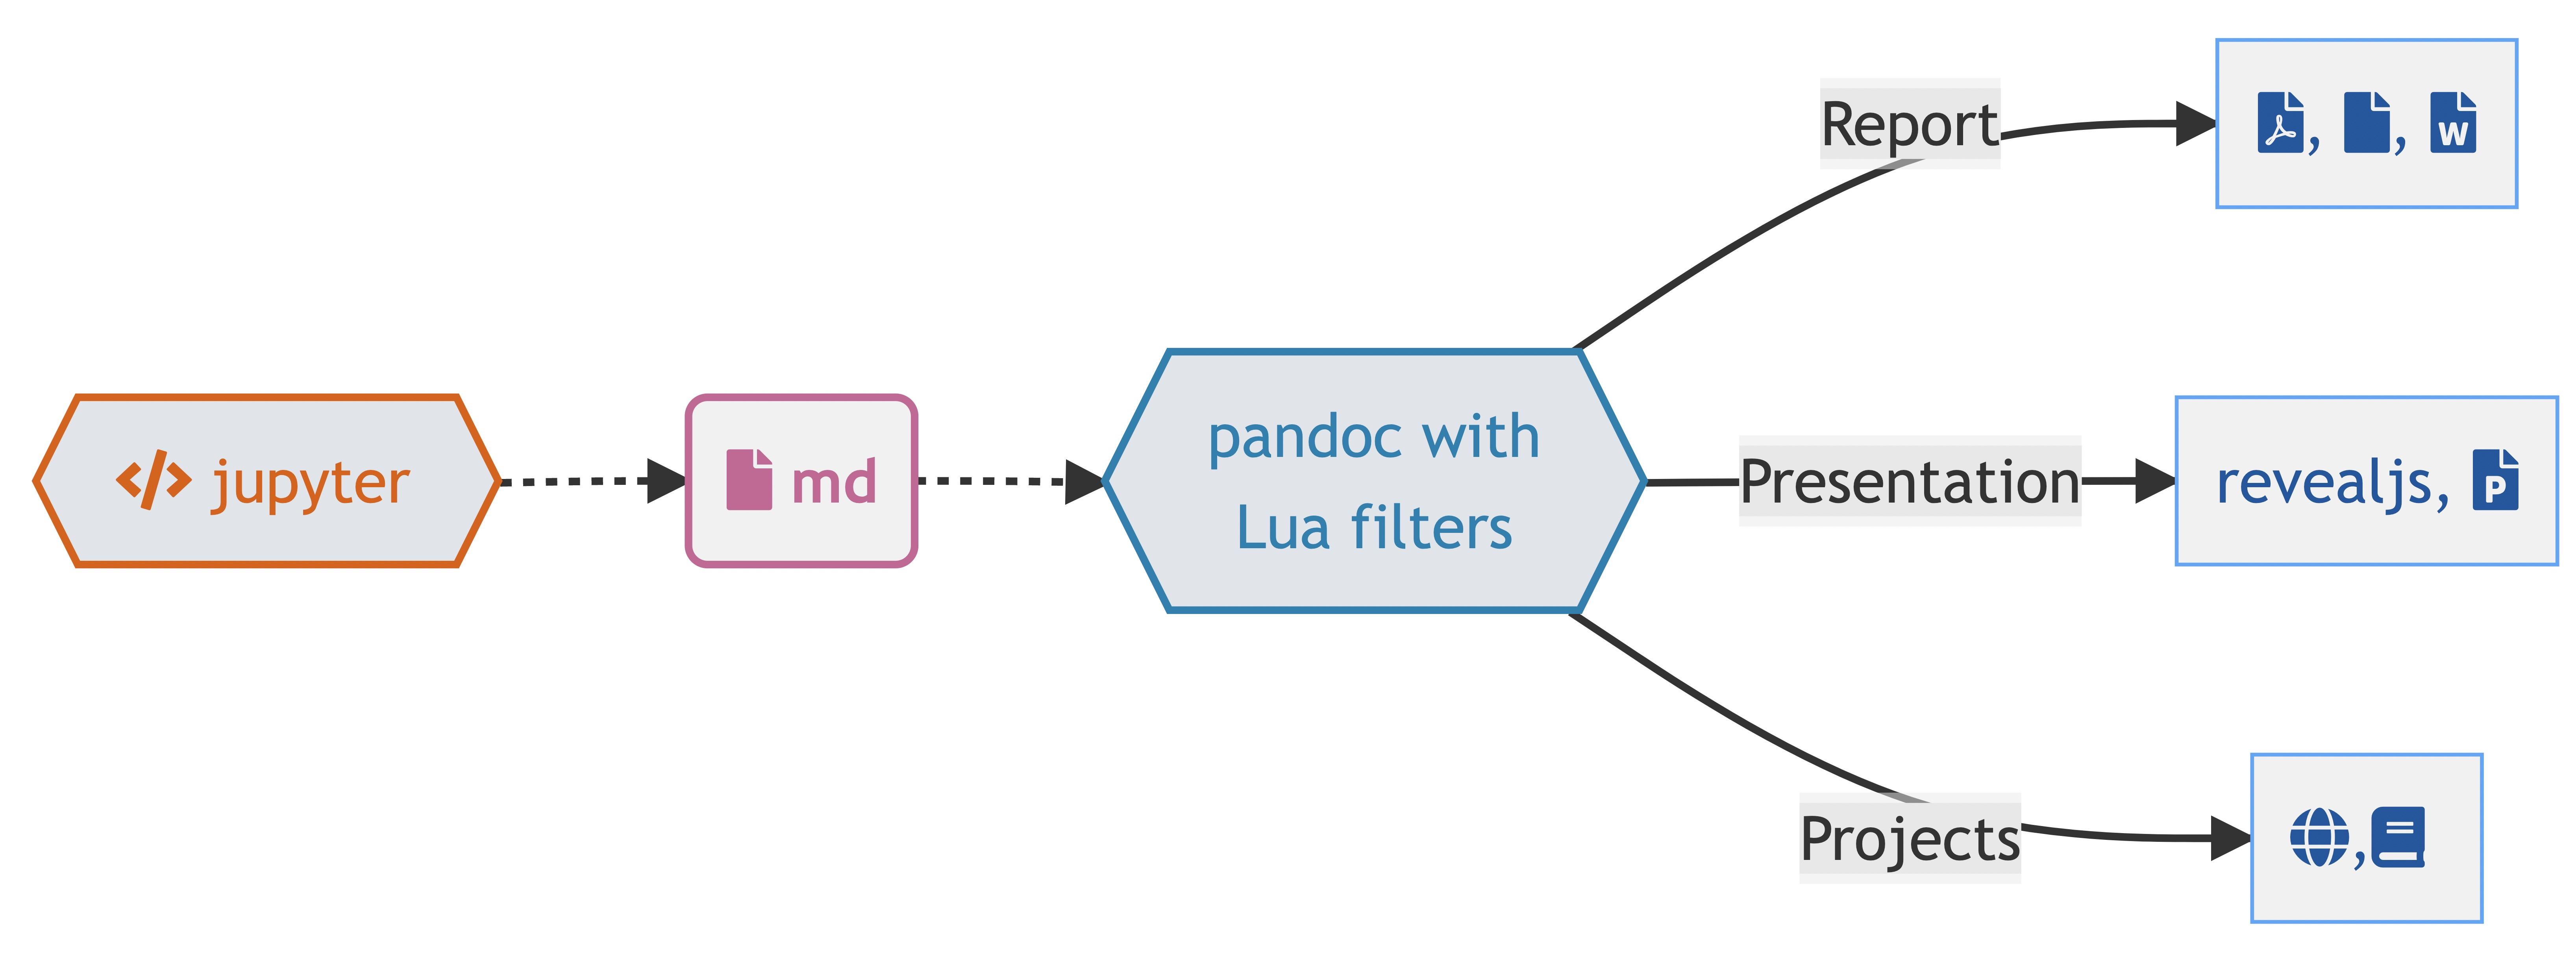
\includegraphics{images/jupyter-alone.jpeg}

\hypertarget{quarto-more-internals}{%
\subsection{Quarto, more internals}\label{quarto-more-internals}}

\begin{itemize}
\tightlist
\item
  Quarto uses an engine like \texttt{knitr} to execute code and generate
  a temporary output \texttt{.md}
\end{itemize}

. . .

The \texttt{.md} file is processed via Pandoc and Quarto's Lua filters +
Bootstrap CSS for HTML or LaTeX for PDF and converted to a final output
format

. . .

Lua filters written by R/Python/Julia developers should be
interchangeable between formats - typically not language specific!

\hypertarget{so-what-is-quarto}{%
\subsection{So what is Quarto?}\label{so-what-is-quarto}}

\begin{quote}
Quarto is a command line interface (CLI) that renders plain text formats
(\texttt{.qmd}, \texttt{.rmd}, \texttt{.md}) OR mixed formats
(\texttt{.ipynb}/Jupyter notebook) into static PDF/Word/HTML reports,
books, websites, presentations and more
\end{quote}

\hypertarget{rstudio-visual-editor}{%
\subsection{RStudio Visual Editor}\label{rstudio-visual-editor}}

\includegraphics{https://quarto.org/docs/visual-editor/images/visual-editing.png}

\hypertarget{one-install-batteries-included}{%
\subsection{One install, ``Batteries
included''}\label{one-install-batteries-included}}

\begin{itemize}
\item
  Quarto is bundled and comes pre-installed with RStudio
  \href{https://www.rstudio.com/products/rstudio/download/\#download}{v2022.07.1}
  and beyond!
\item
  \href{https://quarto.org/docs/computations/r.html\#chunk-options}{more
  infos}
\end{itemize}

\hypertarget{rendering}{%
\subsection{Rendering}\label{rendering}}

\begin{figure}

{\centering \includegraphics[width=10.41667in,height=\textheight]{https://quarto.org/docs/tools/images/rstudio-render.png}

}

\end{figure}

. . .

\begin{enumerate}
\def\labelenumi{\arabic{enumi}.}
\setcounter{enumi}{1}
\tightlist
\item
  System shell via \texttt{quarto\ render}
\end{enumerate}

\textbf{terminal}

\begin{Shaded}
\begin{Highlighting}[]
\ExtensionTok{quarto}\NormalTok{ render document.qmd }\CommentTok{\# defaults to html}
\ExtensionTok{quarto}\NormalTok{ render document.qmd }\AttributeTok{{-}{-}to}\NormalTok{ pdf}
\ExtensionTok{quarto}\NormalTok{ render document.qmd }\AttributeTok{{-}{-}to}\NormalTok{ docx}
\end{Highlighting}
\end{Shaded}

. . .

\begin{enumerate}
\def\labelenumi{\arabic{enumi}.}
\setcounter{enumi}{2}
\tightlist
\item
  R console via \texttt{quarto} R package
\end{enumerate}

\begin{Shaded}
\begin{Highlighting}[]
\FunctionTok{library}\NormalTok{(quarto)}
\FunctionTok{quarto\_render}\NormalTok{(}\StringTok{"document.qmd"}\NormalTok{) }\CommentTok{\# defaults to html}
\FunctionTok{quarto\_render}\NormalTok{(}\StringTok{"document.qmd"}\NormalTok{, }\AttributeTok{output\_format =} \StringTok{"pdf"}\NormalTok{)}
\end{Highlighting}
\end{Shaded}

\hypertarget{change-your-mental-model}{%
\subsection{Change your mental model}\label{change-your-mental-model}}

Source

\begin{figure}

{\centering 
\includegraphics[width=4.6875in,height=\textheight]{images/word.png}

}

\end{figure}

Output

\begin{figure}

{\centering 
\includegraphics[width=4.6875in,height=\textheight]{images/word.png}

}

\end{figure}

\hypertarget{change-your-mental-model-1}{%
\subsection{Change your mental model}\label{change-your-mental-model-1}}

\begin{Shaded}
\begin{Highlighting}[]
\CommentTok{{-}{-}{-}}
\AnnotationTok{title:}\CommentTok{ "ggplot2 demo"}
\AnnotationTok{author:}\CommentTok{ "Norah Jones"}
\AnnotationTok{date:}\CommentTok{ "5/22/2021"}
\AnnotationTok{format:}\CommentTok{ }
\CommentTok{  html:}
\CommentTok{    fig{-}width: 8}
\CommentTok{    fig{-}height: 4}
\CommentTok{    code{-}fold: true}
\CommentTok{{-}{-}{-}}

\FunctionTok{\#\# Air Quality}

\NormalTok{@fig{-}airquality further explores the impact of temperature }
\NormalTok{  on ozone level.}

\InformationTok{\textasciigrave{}\textasciigrave{}\textasciigrave{}\{r\}}
\CommentTok{\#| label: fig{-}airquality}
\CommentTok{\#| fig{-}cap: Temperature and ozone level.}
\CommentTok{\#| warning: false}
\FunctionTok{library}\NormalTok{(ggplot2)}
\FunctionTok{ggplot}\NormalTok{(airquality, }\FunctionTok{aes}\NormalTok{(Temp, Ozone)) }\SpecialCharTok{+} 
  \FunctionTok{geom\_point}\NormalTok{() }\SpecialCharTok{+} 
  \FunctionTok{geom\_smooth}\NormalTok{(}\AttributeTok{method =} \StringTok{"loess"}
\NormalTok{)}
\InformationTok{\textasciigrave{}\textasciigrave{}\textasciigrave{}}
\end{Highlighting}
\end{Shaded}

\includegraphics{https://quarto.org/images/hello-knitr.png}

\hypertarget{a-.qmd-is-a-plain-text-file}{%
\subsection{\texorpdfstring{A \texttt{.qmd} is a plain text
file}{A .qmd is a plain text file}}\label{a-.qmd-is-a-plain-text-file}}

. . .

\begin{itemize}
\tightlist
\item
  Metadata (YAML)
\end{itemize}

\begin{Shaded}
\begin{Highlighting}[]
\FunctionTok{format}\KeywordTok{:}\AttributeTok{ html}
\FunctionTok{engine}\KeywordTok{:}\AttributeTok{ knitr}
\end{Highlighting}
\end{Shaded}

\begin{Shaded}
\begin{Highlighting}[]
\FunctionTok{format}\KeywordTok{:}\AttributeTok{ html}
\FunctionTok{engine}\KeywordTok{:}\AttributeTok{ jupyter}
\end{Highlighting}
\end{Shaded}

. . .

\begin{itemize}
\tightlist
\item
  Code
\end{itemize}

\begin{Shaded}
\begin{Highlighting}[]
\InformationTok{\textasciigrave{}\textasciigrave{}\textasciigrave{}\{r\}}
\FunctionTok{library}\NormalTok{(dplyr)}
\NormalTok{mtcars }\SpecialCharTok{|\textgreater{}} 
  \FunctionTok{group\_by}\NormalTok{(cyl) }\SpecialCharTok{|\textgreater{}} 
  \FunctionTok{summarize}\NormalTok{(}\AttributeTok{mean =} \FunctionTok{mean}\NormalTok{(mpg))}
\InformationTok{\textasciigrave{}\textasciigrave{}\textasciigrave{}}
\end{Highlighting}
\end{Shaded}

\begin{Shaded}
\begin{Highlighting}[]
\InformationTok{\textasciigrave{}\textasciigrave{}\textasciigrave{}\{python\}}
\ImportTok{from}\NormalTok{ siuba }\ImportTok{import} \OperatorTok{*}
\NormalTok{(mtcars}
  \OperatorTok{\textgreater{}\textgreater{}}\NormalTok{ group\_by(\_.cyl)}
  \OperatorTok{\textgreater{}\textgreater{}}\NormalTok{ summarize(avg\_mpg }\OperatorTok{=}\NormalTok{ \_.mpg.mean()))}
\InformationTok{\textasciigrave{}\textasciigrave{}\textasciigrave{}}
\end{Highlighting}
\end{Shaded}

. . .

\begin{itemize}
\tightlist
\item
  Text
\end{itemize}

\begin{Shaded}
\begin{Highlighting}[]
\FunctionTok{\# Heading 1}
\NormalTok{This is a sentence with some **bold text**, *italic text* and an }
\AlertTok{![image](image.png)}\NormalTok{\{fig{-}alt="Alt text for this image"\}.}
\end{Highlighting}
\end{Shaded}

\hypertarget{metadata-yaml}{%
\subsection{Metadata: YAML}\label{metadata-yaml}}

The \href{https://yaml.org/}{YAML} metadata or header is:

\begin{quote}
processed in many stages of the rendering process and can influence the
final document in many different ways. It is placed at the very
beginning of the document and is read by each of Pandoc, Quarto and
\texttt{knitr}. Along the way, the information that it contains can
affect the code, content, and the rendering process. \#\# YAML
\end{quote}

\begin{Shaded}
\begin{Highlighting}[]
\PreprocessorTok{{-}{-}{-}}
\FunctionTok{title}\KeywordTok{:}\AttributeTok{ }\StringTok{"My Document"}
\FunctionTok{format}\KeywordTok{:}\AttributeTok{ }
\AttributeTok{  }\FunctionTok{html}\KeywordTok{:}
\AttributeTok{    }\FunctionTok{toc}\KeywordTok{:}\AttributeTok{ }\CharTok{true}
\AttributeTok{    }\FunctionTok{code{-}fold}\KeywordTok{:}\AttributeTok{ }\CharTok{true}
\PreprocessorTok{{-}{-}{-}}
\end{Highlighting}
\end{Shaded}

\hypertarget{markdown}{%
\subsection{Markdown}\label{markdown}}

\begin{quote}
Quarto is based on Pandoc and uses its variation of markdown as its
underlying document syntax. Pandoc markdown is an extended and slightly
revised version of John Gruber's
\href{https://daringfireball.net/projects/markdown/}{Markdown} syntax. .
. .
\end{quote}

\begin{quote}
Markdown is a plain text format that is designed to be easy to write,
and, even more importantly, easy to read \#\# Text Formatting
\end{quote}

\begin{longtable}[]{@{}
  >{\raggedright\arraybackslash}p{(\columnwidth - 2\tabcolsep) * \real{0.5000}}
  >{\raggedright\arraybackslash}p{(\columnwidth - 2\tabcolsep) * \real{0.4444}}@{}}
\toprule()
\begin{minipage}[b]{\linewidth}\raggedright
Markdown Syntax
\end{minipage} & \begin{minipage}[b]{\linewidth}\raggedright
Output
\end{minipage} \\
\midrule()
\endhead
\begin{minipage}[t]{\linewidth}\raggedright
\begin{verbatim}
*italics* and **bold**
\end{verbatim}
\end{minipage} & \emph{italics} and \textbf{bold} \\
\begin{minipage}[t]{\linewidth}\raggedright
\begin{verbatim}
superscript^2^ / subscript~2~
\end{verbatim}
\end{minipage} & superscript\textsuperscript{2} /
subscript\textsubscript{2} \\
\begin{minipage}[t]{\linewidth}\raggedright
\begin{verbatim}
~~strikethrough~~
\end{verbatim}
\end{minipage} & \sout{strikethrough} \\
\begin{minipage}[t]{\linewidth}\raggedright
\begin{verbatim}
`verbatim code`
\end{verbatim}
\end{minipage} & \texttt{verbatim\ code} \\
\bottomrule()
\end{longtable}

\hypertarget{headings}{%
\subsection{Headings}\label{headings}}

\begin{longtable}[]{@{}
  >{\raggedright\arraybackslash}p{(\columnwidth - 2\tabcolsep) * \real{0.3056}}
  >{\raggedright\arraybackslash}p{(\columnwidth - 2\tabcolsep) * \real{0.2500}}@{}}
\toprule()
\begin{minipage}[b]{\linewidth}\raggedright
Markdown Syntax
\end{minipage} & \begin{minipage}[b]{\linewidth}\raggedright
Output
\end{minipage} \\
\midrule()
\endhead
\begin{minipage}[t]{\linewidth}\raggedright
\begin{verbatim}
# Header 1
\end{verbatim}
\end{minipage} & \begin{minipage}[t]{\linewidth}\raggedright
\hypertarget{header-1}{%
\section{Header 1}\label{header-1}}
\end{minipage} \\
\begin{minipage}[t]{\linewidth}\raggedright
\begin{verbatim}
## Header 2
\end{verbatim}
\end{minipage} & \begin{minipage}[t]{\linewidth}\raggedright
\hypertarget{header-2}{%
\subsection{Header 2}\label{header-2}}
\end{minipage} \\
\begin{minipage}[t]{\linewidth}\raggedright
\begin{verbatim}
### Header 3
\end{verbatim}
\end{minipage} & \begin{minipage}[t]{\linewidth}\raggedright
\hypertarget{header-3}{%
\subsubsection{Header 3}\label{header-3}}
\end{minipage} \\
\begin{minipage}[t]{\linewidth}\raggedright
\begin{verbatim}
#### Header 4
\end{verbatim}
\end{minipage} & \begin{minipage}[t]{\linewidth}\raggedright
\hypertarget{header-4}{%
\paragraph{Header 4}\label{header-4}}
\end{minipage} \\
\begin{minipage}[t]{\linewidth}\raggedright
\begin{verbatim}
##### Header 5
\end{verbatim}
\end{minipage} & \begin{minipage}[t]{\linewidth}\raggedright
\hypertarget{header-5}{%
\subparagraph{Header 5}\label{header-5}}
\end{minipage} \\
\begin{minipage}[t]{\linewidth}\raggedright
\begin{verbatim}
###### Header 6
\end{verbatim}
\end{minipage} & \begin{minipage}[t]{\linewidth}\raggedright
Header 6
\end{minipage} \\
\bottomrule()
\end{longtable}

\hypertarget{code}{%
\subsection{Code}\label{code}}

\begin{Shaded}
\begin{Highlighting}[]
\InformationTok{\textasciigrave{}\textasciigrave{}\textasciigrave{}\{r\}}
\CommentTok{\#| output{-}location: column}
\CommentTok{\#| label: fig{-}airquality}
\CommentTok{\#| fig{-}cap: Temperature and ozone level.}
\CommentTok{\#| warning: false}
\FunctionTok{library}\NormalTok{(ggplot2)}
\FunctionTok{ggplot}\NormalTok{(airquality, }\FunctionTok{aes}\NormalTok{(Temp, Ozone)) }\SpecialCharTok{+} 
  \FunctionTok{geom\_point}\NormalTok{() }\SpecialCharTok{+} 
  \FunctionTok{geom\_smooth}\NormalTok{(}\AttributeTok{method =} \StringTok{"loess"}
\NormalTok{)}
\InformationTok{\textasciigrave{}\textasciigrave{}\textasciigrave{}}
\end{Highlighting}
\end{Shaded}

\begin{figure}[H]

{\centering 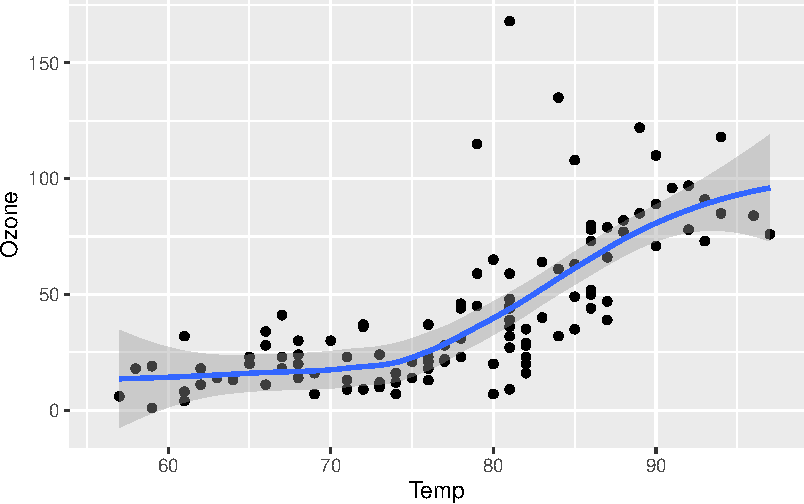
\includegraphics{slides_files/figure-pdf/fig-airquality-1.pdf}

}

\caption{\label{fig-airquality}Temperature and ozone level.}

\end{figure}

\hypertarget{code-more-than-just-r}{%
\subsection{Code, more than just R}\label{code-more-than-just-r}}

\begin{Shaded}
\begin{Highlighting}[]
\InformationTok{\textasciigrave{}\textasciigrave{}\textasciigrave{}\{python\}}
\CommentTok{\#| eval: false}
\CommentTok{\#| label: fig{-}polar}
\CommentTok{\#| fig{-}cap: "A line plot on a polar axis"}
\ImportTok{import}\NormalTok{ numpy }\ImportTok{as}\NormalTok{ np}
\ImportTok{import}\NormalTok{ matplotlib.pyplot }\ImportTok{as}\NormalTok{ plt}
\NormalTok{r }\OperatorTok{=}\NormalTok{ np.arange(}\DecValTok{0}\NormalTok{, }\DecValTok{2}\NormalTok{, }\FloatTok{0.01}\NormalTok{)}
\NormalTok{theta }\OperatorTok{=} \DecValTok{2} \OperatorTok{*}\NormalTok{ np.pi }\OperatorTok{*}\NormalTok{ r}
\NormalTok{fig, ax }\OperatorTok{=}\NormalTok{ plt.subplots(}
\NormalTok{  subplot\_kw }\OperatorTok{=}\NormalTok{ \{}\StringTok{\textquotesingle{}projection\textquotesingle{}}\NormalTok{: }\StringTok{\textquotesingle{}polar\textquotesingle{}}\NormalTok{\} }
\NormalTok{)}
\NormalTok{ax.plot(theta, r)}
\NormalTok{ax.set\_rticks([}\FloatTok{0.5}\NormalTok{, }\DecValTok{1}\NormalTok{, }\FloatTok{1.5}\NormalTok{, }\DecValTok{2}\NormalTok{])}
\NormalTok{ax.grid(}\VariableTok{True}\NormalTok{)}
\NormalTok{plt.show()}
\InformationTok{\textasciigrave{}\textasciigrave{}\textasciigrave{}}
\end{Highlighting}
\end{Shaded}

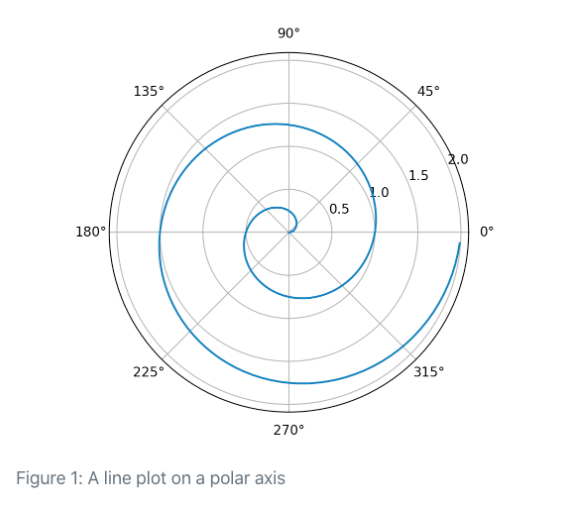
\includegraphics[width=6.77083in,height=\textheight]{images/polar-axis.png}



\end{document}
